% Options for packages loaded elsewhere
\PassOptionsToPackage{unicode}{hyperref}
\PassOptionsToPackage{hyphens}{url}
%
\documentclass[
]{article}
\usepackage{amsmath,amssymb}
\usepackage{iftex}
\ifPDFTeX
  \usepackage[T1]{fontenc}
  \usepackage[utf8]{inputenc}
  \usepackage{textcomp} % provide euro and other symbols
\else % if luatex or xetex
  \usepackage{unicode-math} % this also loads fontspec
  \defaultfontfeatures{Scale=MatchLowercase}
  \defaultfontfeatures[\rmfamily]{Ligatures=TeX,Scale=1}
\fi
\usepackage{lmodern}
\ifPDFTeX\else
  % xetex/luatex font selection
\fi
% Use upquote if available, for straight quotes in verbatim environments
\IfFileExists{upquote.sty}{\usepackage{upquote}}{}
\IfFileExists{microtype.sty}{% use microtype if available
  \usepackage[]{microtype}
  \UseMicrotypeSet[protrusion]{basicmath} % disable protrusion for tt fonts
}{}
\makeatletter
\@ifundefined{KOMAClassName}{% if non-KOMA class
  \IfFileExists{parskip.sty}{%
    \usepackage{parskip}
  }{% else
    \setlength{\parindent}{0pt}
    \setlength{\parskip}{6pt plus 2pt minus 1pt}}
}{% if KOMA class
  \KOMAoptions{parskip=half}}
\makeatother
\usepackage{xcolor}
\usepackage[margin=1in]{geometry}
\usepackage{color}
\usepackage{fancyvrb}
\newcommand{\VerbBar}{|}
\newcommand{\VERB}{\Verb[commandchars=\\\{\}]}
\DefineVerbatimEnvironment{Highlighting}{Verbatim}{commandchars=\\\{\}}
% Add ',fontsize=\small' for more characters per line
\usepackage{framed}
\definecolor{shadecolor}{RGB}{248,248,248}
\newenvironment{Shaded}{\begin{snugshade}}{\end{snugshade}}
\newcommand{\AlertTok}[1]{\textcolor[rgb]{0.94,0.16,0.16}{#1}}
\newcommand{\AnnotationTok}[1]{\textcolor[rgb]{0.56,0.35,0.01}{\textbf{\textit{#1}}}}
\newcommand{\AttributeTok}[1]{\textcolor[rgb]{0.13,0.29,0.53}{#1}}
\newcommand{\BaseNTok}[1]{\textcolor[rgb]{0.00,0.00,0.81}{#1}}
\newcommand{\BuiltInTok}[1]{#1}
\newcommand{\CharTok}[1]{\textcolor[rgb]{0.31,0.60,0.02}{#1}}
\newcommand{\CommentTok}[1]{\textcolor[rgb]{0.56,0.35,0.01}{\textit{#1}}}
\newcommand{\CommentVarTok}[1]{\textcolor[rgb]{0.56,0.35,0.01}{\textbf{\textit{#1}}}}
\newcommand{\ConstantTok}[1]{\textcolor[rgb]{0.56,0.35,0.01}{#1}}
\newcommand{\ControlFlowTok}[1]{\textcolor[rgb]{0.13,0.29,0.53}{\textbf{#1}}}
\newcommand{\DataTypeTok}[1]{\textcolor[rgb]{0.13,0.29,0.53}{#1}}
\newcommand{\DecValTok}[1]{\textcolor[rgb]{0.00,0.00,0.81}{#1}}
\newcommand{\DocumentationTok}[1]{\textcolor[rgb]{0.56,0.35,0.01}{\textbf{\textit{#1}}}}
\newcommand{\ErrorTok}[1]{\textcolor[rgb]{0.64,0.00,0.00}{\textbf{#1}}}
\newcommand{\ExtensionTok}[1]{#1}
\newcommand{\FloatTok}[1]{\textcolor[rgb]{0.00,0.00,0.81}{#1}}
\newcommand{\FunctionTok}[1]{\textcolor[rgb]{0.13,0.29,0.53}{\textbf{#1}}}
\newcommand{\ImportTok}[1]{#1}
\newcommand{\InformationTok}[1]{\textcolor[rgb]{0.56,0.35,0.01}{\textbf{\textit{#1}}}}
\newcommand{\KeywordTok}[1]{\textcolor[rgb]{0.13,0.29,0.53}{\textbf{#1}}}
\newcommand{\NormalTok}[1]{#1}
\newcommand{\OperatorTok}[1]{\textcolor[rgb]{0.81,0.36,0.00}{\textbf{#1}}}
\newcommand{\OtherTok}[1]{\textcolor[rgb]{0.56,0.35,0.01}{#1}}
\newcommand{\PreprocessorTok}[1]{\textcolor[rgb]{0.56,0.35,0.01}{\textit{#1}}}
\newcommand{\RegionMarkerTok}[1]{#1}
\newcommand{\SpecialCharTok}[1]{\textcolor[rgb]{0.81,0.36,0.00}{\textbf{#1}}}
\newcommand{\SpecialStringTok}[1]{\textcolor[rgb]{0.31,0.60,0.02}{#1}}
\newcommand{\StringTok}[1]{\textcolor[rgb]{0.31,0.60,0.02}{#1}}
\newcommand{\VariableTok}[1]{\textcolor[rgb]{0.00,0.00,0.00}{#1}}
\newcommand{\VerbatimStringTok}[1]{\textcolor[rgb]{0.31,0.60,0.02}{#1}}
\newcommand{\WarningTok}[1]{\textcolor[rgb]{0.56,0.35,0.01}{\textbf{\textit{#1}}}}
\usepackage{graphicx}
\makeatletter
\def\maxwidth{\ifdim\Gin@nat@width>\linewidth\linewidth\else\Gin@nat@width\fi}
\def\maxheight{\ifdim\Gin@nat@height>\textheight\textheight\else\Gin@nat@height\fi}
\makeatother
% Scale images if necessary, so that they will not overflow the page
% margins by default, and it is still possible to overwrite the defaults
% using explicit options in \includegraphics[width, height, ...]{}
\setkeys{Gin}{width=\maxwidth,height=\maxheight,keepaspectratio}
% Set default figure placement to htbp
\makeatletter
\def\fps@figure{htbp}
\makeatother
\setlength{\emergencystretch}{3em} % prevent overfull lines
\providecommand{\tightlist}{%
  \setlength{\itemsep}{0pt}\setlength{\parskip}{0pt}}
\setcounter{secnumdepth}{-\maxdimen} % remove section numbering
\ifLuaTeX
  \usepackage{selnolig}  % disable illegal ligatures
\fi
\IfFileExists{bookmark.sty}{\usepackage{bookmark}}{\usepackage{hyperref}}
\IfFileExists{xurl.sty}{\usepackage{xurl}}{} % add URL line breaks if available
\urlstyle{same}
\hypersetup{
  pdftitle={Stats Lab 7},
  pdfauthor={Wynona},
  hidelinks,
  pdfcreator={LaTeX via pandoc}}

\title{Stats Lab 7}
\author{Wynona}
\date{2024-02-28}

\begin{document}
\maketitle

\hypertarget{question-1}{%
\subsection{QUESTION 1:}\label{question-1}}

Start by fitting an intercept-only model: agb = beta0 + epsilon, epsilon
∼ N (0, sigma2I) Call this model `fit\_1'. a. Report the value of beta0.
How does it compare to the sample mean of agb? b. What is the standard
error? How does it compare to the standard error of the sample mean?

\begin{Shaded}
\begin{Highlighting}[]
\CommentTok{\#Q1a)}
\NormalTok{AGB.df}\OtherTok{\textless{}{-}}\FunctionTok{read.csv}\NormalTok{(}\StringTok{"\textasciitilde{}/ENV 872/EDA\_Spring2024/Misc./agb.csv"}\NormalTok{, }\AttributeTok{header=}\NormalTok{T)}

\FunctionTok{colnames}\NormalTok{(AGB.df)}
\end{Highlighting}
\end{Shaded}

\begin{verbatim}
## [1] "growth"     "state"      "basal_area" "agb"
\end{verbatim}

\begin{Shaded}
\begin{Highlighting}[]
\NormalTok{fit\_1}\OtherTok{\textless{}{-}}\FunctionTok{lm}\NormalTok{(agb}\SpecialCharTok{\textasciitilde{}} \DecValTok{1}\NormalTok{, AGB.df)}
\FunctionTok{summary}\NormalTok{(fit\_1)}
\end{Highlighting}
\end{Shaded}

\begin{verbatim}
## 
## Call:
## lm(formula = agb ~ 1, data = AGB.df)
## 
## Residuals:
##      Min       1Q   Median       3Q      Max 
## -234.938  -64.967   -5.102   72.674  311.866 
## 
## Coefficients:
##             Estimate Std. Error t value Pr(>|t|)    
## (Intercept)  410.733      6.482   63.36   <2e-16 ***
## ---
## Signif. codes:  0 '***' 0.001 '**' 0.01 '*' 0.05 '.' 0.1 ' ' 1
## 
## Residual standard error: 102.5 on 249 degrees of freedom
\end{verbatim}

\begin{Shaded}
\begin{Highlighting}[]
\FunctionTok{mean}\NormalTok{(AGB.df}\SpecialCharTok{$}\NormalTok{agb)}
\end{Highlighting}
\end{Shaded}

\begin{verbatim}
## [1] 410.7327
\end{verbatim}

\begin{Shaded}
\begin{Highlighting}[]
\CommentTok{\#Q1b)}
\FunctionTok{sd}\NormalTok{(AGB.df}\SpecialCharTok{$}\NormalTok{agb)}
\end{Highlighting}
\end{Shaded}

\begin{verbatim}
## [1] 102.4953
\end{verbatim}

\begin{enumerate}
\def\labelenumi{\alph{enumi})}
\tightlist
\item
  The value of beta0 is -234.938 The sample mean of agb is 410.7327
  which is much higher than the value of beta0.
\item
  The standard error of the intercept is 6.482. The sample standard
  error is 102.4953 which is much higher.
\end{enumerate}

\hypertarget{question-2}{%
\subsection{QUESTION 2}\label{question-2}}

Now suppose you hypothesize that AGB differs between old-growth and
new-growth forests. Create a binary indicator variable from the growth
variable. Code this variable as 1 if the sample is from an old growth
forest, and 0 otherwise.

\begin{Shaded}
\begin{Highlighting}[]
\NormalTok{AGB.df}\OtherTok{\textless{}{-}}\NormalTok{ AGB.df}\SpecialCharTok{\%\textgreater{}\%}
  \FunctionTok{mutate}\NormalTok{(}\AttributeTok{old.growth =} \FunctionTok{ifelse}\NormalTok{(growth }\SpecialCharTok{==}\StringTok{"Old Growth"}\NormalTok{,}\DecValTok{1}\NormalTok{,}\DecValTok{0}\NormalTok{))}
\end{Highlighting}
\end{Shaded}

Next, expand on the model above by including this new indicator
variable, as follows: agb = beta0 + old.growth × beta1 + epsilon,
epsilon ∼ N (0, sigma2I) Call this model `fit\_2'.

\begin{Shaded}
\begin{Highlighting}[]
\NormalTok{fit\_2}\OtherTok{\textless{}{-}}\FunctionTok{lm}\NormalTok{(agb}\SpecialCharTok{\textasciitilde{}}\NormalTok{ old.growth, AGB.df)}
\FunctionTok{summary}\NormalTok{(fit\_2)}
\end{Highlighting}
\end{Shaded}

\begin{verbatim}
## 
## Call:
## lm(formula = agb ~ old.growth, data = AGB.df)
## 
## Residuals:
##     Min      1Q  Median      3Q     Max 
## -281.45  -55.02    3.59   54.92  347.54 
## 
## Coefficients:
##             Estimate Std. Error t value Pr(>|t|)    
## (Intercept)  363.469      8.197  44.342  < 2e-16 ***
## old.growth    93.778     11.546   8.122 2.16e-14 ***
## ---
## Signif. codes:  0 '***' 0.001 '**' 0.01 '*' 0.05 '.' 0.1 ' ' 1
## 
## Residual standard error: 91.28 on 248 degrees of freedom
## Multiple R-squared:  0.2101, Adjusted R-squared:  0.2069 
## F-statistic: 65.97 on 1 and 248 DF,  p-value: 2.163e-14
\end{verbatim}

\begin{enumerate}
\def\labelenumi{\alph{enumi}.}
\item
  Report the value of beta0. How does it compare to the sample mean of
  abg among new-growth forest? \textgreater{} Answer: beta0 is 363.469.
  THe sample mean of abg among new-growth forests are the same.
\item
  Report the difference in means between AGB among samples from
  old-growth forests and new-growth forests. Calculate the difference as
  the mean of AGB in old-growth forests minus the mean of AGB in
  new-growth forests. \textgreater{} Answer: The difference in means
  between AGB among old vs.~new-growth forests is 93.778.
\item
  What is the value of the estimate for the old-growth forest?
  \textgreater{} Answer: THe sample mean of abg among old-growth forests
  is 363.469 + 93.778 = 457.247
\end{enumerate}

\begin{Shaded}
\begin{Highlighting}[]
\NormalTok{y}\OtherTok{\textless{}{-}}\FloatTok{363.469} \SpecialCharTok{+} \FloatTok{93.778}
\NormalTok{y}
\end{Highlighting}
\end{Shaded}

\begin{verbatim}
## [1] 457.247
\end{verbatim}

\begin{enumerate}
\def\labelenumi{\alph{enumi}.}
\setcounter{enumi}{3}
\item
  Interpret the estimate of old-growth forest (Do not interpret the
  estimate in terms of a hypothesis test). \textgreater{} Answer: The
  estimate of old-growth forest is the incremental adjustment to the
  intercept that reflects the difference in AGB between old- and
  new-growth forests.
\item
  Conduct a hypothesis test in which the null hypothesis is that there
  is no difference in AGB between new-growth and old-growth forests.
\end{enumerate}

\begin{Shaded}
\begin{Highlighting}[]
\FunctionTok{t.test}\NormalTok{(agb}\SpecialCharTok{\textasciitilde{}}\NormalTok{old.growth, }\AttributeTok{data=}\NormalTok{AGB.df)}
\end{Highlighting}
\end{Shaded}

\begin{verbatim}
## 
##  Welch Two Sample t-test
## 
## data:  agb by old.growth
## t = -8.1323, df = 243.09, p-value = 2.162e-14
## alternative hypothesis: true difference in means between group 0 and group 1 is not equal to 0
## 95 percent confidence interval:
##  -116.49188  -71.06321
## sample estimates:
## mean in group 0 mean in group 1 
##        363.4688        457.2463
\end{verbatim}

\begin{quote}
Answer: After running the t-test, we reject the null hypothesis that
there is no difference in AGB between new and old-growth forests because
the p-value is 2.162e-14 which is way smaller than 0.05.
\end{quote}

\begin{enumerate}
\def\labelenumi{\alph{enumi}.}
\setcounter{enumi}{5}
\tightlist
\item
  Make a scatter plot of the data and add the regression lines: one for
  old growth forest; one for new growth forest. (Hint: the indicator for
  old-growth versus new-growth should be on the x-axis, and AGB on the
  y-axis). Be sure to use a different color for old growth versus new
  growth data points and regression lines (e.g.~dark green for old
  growth data points and regression line and blue for new growth data
  points and regression line).
\end{enumerate}

\begin{Shaded}
\begin{Highlighting}[]
\FunctionTok{colnames}\NormalTok{(AGB.df)}
\end{Highlighting}
\end{Shaded}

\begin{verbatim}
## [1] "growth"     "state"      "basal_area" "agb"        "old.growth"
\end{verbatim}

\begin{Shaded}
\begin{Highlighting}[]
\FunctionTok{ggplot}\NormalTok{(AGB.df, }\FunctionTok{aes}\NormalTok{(old.growth, agb))}\SpecialCharTok{+}\FunctionTok{geom\_point}\NormalTok{(}\FunctionTok{aes}\NormalTok{(}\AttributeTok{col=}\NormalTok{old.growth))}\SpecialCharTok{+} \FunctionTok{geom\_line}\NormalTok{(}\FunctionTok{aes}\NormalTok{(}\AttributeTok{col=}\NormalTok{old.growth))}
\end{Highlighting}
\end{Shaded}

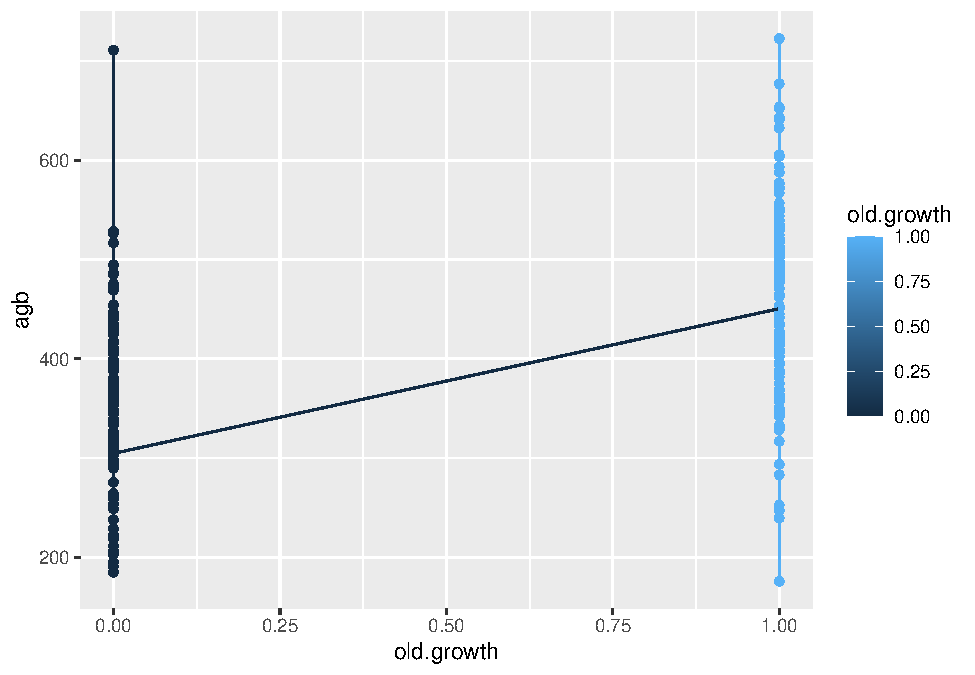
\includegraphics{Stats-Lab-7-FINAL_files/figure-latex/unnamed-chunk-4-1.pdf}

\hypertarget{question-3}{%
\subsection{Question 3}\label{question-3}}

Now suppose you are interested in understanding whether or not basal
area is associated with AGB. Now fit a simple linear regression of the
following form: y = beta0 + basal.areabeta1 + epsilon, epsilon ∼ N (0,
sigma2I). Call this model `fit\_3'

\begin{Shaded}
\begin{Highlighting}[]
\NormalTok{fit\_3 }\OtherTok{\textless{}{-}}\FunctionTok{lm}\NormalTok{(agb }\SpecialCharTok{\textasciitilde{}}\NormalTok{ basal\_area, AGB.df)}
\end{Highlighting}
\end{Shaded}

\begin{enumerate}
\def\labelenumi{\alph{enumi}.}
\item
  Report the value of beta0 and interpret its meaning.
  \textgreater Answer: beta0 is -113.38. This suggests that when basal
  area is 0, above ground biomass is -113.38. {[}ADD UNITS{]}
\item
  Report the value of beta1 and interpret its meaning (not in terms of a
  hypothesis test, but substantively). \textgreater Answer: beta1 is
  18.89, which means that as basal\_area increases by 1, the above
  ground biomass increases by 18.89. {[}ADD UNITS{]}
\item
  Now define a new variable called `basal.area.centered' in which you
  subtract the mean basal area from each observation of `basal.area'.
  Refit the above model. Report the new value of beta0 and interpret its
  meaning.
\end{enumerate}

\begin{Shaded}
\begin{Highlighting}[]
\FunctionTok{colnames}\NormalTok{(AGB.df)}
\end{Highlighting}
\end{Shaded}

\begin{verbatim}
## [1] "growth"     "state"      "basal_area" "agb"        "old.growth"
\end{verbatim}

\begin{Shaded}
\begin{Highlighting}[]
\NormalTok{AGB.df}\OtherTok{\textless{}{-}}\NormalTok{ AGB.df}\SpecialCharTok{\%\textgreater{}\%}
  \FunctionTok{mutate}\NormalTok{(}\AttributeTok{basal.area.centered=}\NormalTok{ (basal\_area}\SpecialCharTok{{-}}\FunctionTok{mean}\NormalTok{(basal\_area)))}
\NormalTok{AGB.df}
\end{Highlighting}
\end{Shaded}

\begin{verbatim}
##         growth state basal_area      agb old.growth basal.area.centered
## 1   New Growth    CA   25.61387 366.4559          0         -2.12471446
## 2   Old Growth    WA   29.00405 450.4992          1          1.26546167
## 3   Old Growth    ME   30.98250 507.5905          1          3.24391359
## 4   Old Growth    NC   27.06275 423.7340          1         -0.67583971
## 5   Old Growth    CA   31.35959 510.2132          1          3.62100174
## 6   New Growth    CA   25.80662 326.7147          0         -1.93196970
## 7   New Growth    ME   35.25429 471.8941          0          7.51570716
## 8   Old Growth    ME   27.87633 441.0699          1          0.13774348
## 9   New Growth    ME   28.66158 410.5476          0          0.92299190
## 10  Old Growth    ME   28.96754 512.3449          1          1.22895391
## 11  Old Growth    NC   29.03193 471.4234          1          1.29334616
## 12  Old Growth    CO   33.45055 539.8039          1          5.71196680
## 13  Old Growth    CO   32.92917 529.4163          1          5.19058489
## 14  New Growth    WA   25.45993 297.9366          0         -2.27865237
## 15  Old Growth    CO   27.03652 406.2263          1         -0.70206820
## 16  New Growth    CO   25.03207 308.4956          0         -2.70651656
## 17  Old Growth    WA   30.76127 503.8567          1          3.02268583
## 18  New Growth    CA   31.61415 416.9494          0          3.87556503
## 19  Old Growth    CO   31.82218 517.2337          1          4.08359022
## 20  Old Growth    CA   33.55702 543.9224          1          5.81843192
## 21  New Growth    WA   26.35874 378.8927          0         -1.37984453
## 22  Old Growth    NC   27.75304 395.0702          1          0.01445654
## 23  New Growth    ME   30.60342 469.6590          0          2.86483724
## 24  Old Growth    CA   34.67562 575.8593          1          6.93703732
## 25  New Growth    ME   26.40814 356.8920          0         -1.33044348
## 26  New Growth    NC   31.08576 424.6977          0          3.34717158
## 27  Old Growth    ME   38.94367 676.9774          1         11.20508584
## 28  Old Growth    CA   22.21053 345.4421          1         -5.52805397
## 29  Old Growth    ME   18.17766 293.7682          1         -9.56092683
## 30  Old Growth    CA   25.46067 402.2109          1         -2.27791674
## 31  New Growth    CA   27.27092 369.7658          0         -0.46766017
## 32  New Growth    CO   15.55381 195.0143          0        -12.18477363
## 33  Old Growth    CO   23.44240 330.4892          1         -4.29618111
## 34  Old Growth    WA   30.90025 513.3541          1          3.16166490
## 35  New Growth    ME   28.34553 405.0344          0          0.60694602
## 36  Old Growth    CO   24.75795 358.5820          1         -2.98063896
## 37  New Growth    ME   25.95863 333.7334          0         -1.77995691
## 38  New Growth    NC   31.91934 428.9095          0          4.18075804
## 39  Old Growth    WA   25.94341 413.2952          1         -1.79517313
## 40  New Growth    NC   16.26361 184.9748          0        -11.47497199
## 41  New Growth    NC   27.59028 374.7458          0         -0.14830103
## 42  New Growth    NC   33.63643 475.5577          0          5.89784555
## 43  New Growth    CO   29.37078 378.9356          0          1.63219797
## 44  Old Growth    ME   23.81231 368.9803          1         -3.92627156
## 45  Old Growth    CA   30.91210 501.3294          1          3.17351128
## 46  New Growth    WA   24.41512 323.2212          0         -3.32346023
## 47  Old Growth    NC   22.56516 328.3556          1         -5.17342888
## 48  Old Growth    CA   26.49954 409.6635          1         -1.23904776
## 49  New Growth    CA   28.80193 362.8434          0          1.06334980
## 50  New Growth    CO   18.97534 222.6564          0         -8.76324065
## 51  New Growth    CA   22.27696 297.8171          0         -5.46162707
## 52  New Growth    WA   22.30393 259.1295          0         -5.43465459
## 53  New Growth    ME   27.40931 378.6808          0         -0.32927171
## 54  New Growth    CO   26.14963 293.7348          0         -1.58895405
## 55  Old Growth    CO   25.04390 385.4362          1         -2.69468423
## 56  New Growth    NC   22.57008 303.1707          0         -5.16850743
## 57  New Growth    NC   24.17914 315.1686          0         -3.55944272
## 58  Old Growth    ME   22.51716 359.8904          1         -5.22142297
## 59  New Growth    WA   17.64079 202.8966          0        -10.09779227
## 60  Old Growth    WA   35.39086 567.0773          1          7.65227959
## 61  Old Growth    ME   16.62192 252.5557          1        -11.11666860
## 62  Old Growth    CO   14.86709 175.7948          1        -12.87149350
## 63  New Growth    NC   27.98512 371.4783          0          0.24653527
## 64  Old Growth    CA   29.92721 488.4789          1          2.18862264
## 65  New Growth    CO   27.76060 395.4940          0          0.02201513
## 66  New Growth    CO   21.65547 260.0623          0         -6.08311813
## 67  New Growth    ME   16.99232 211.5165          0        -10.74626184
## 68  New Growth    NC   35.24166 469.6152          0          7.50307054
## 69  Old Growth    WA   30.12395 480.7064          1          2.38536711
## 70  Old Growth    CO   31.89014 507.6941          1          4.15155307
## 71  New Growth    ME   25.99443 353.4106          0         -1.74415410
## 72  New Growth    CA   22.99594 325.4990          0         -4.74264489
## 73  New Growth    CA   31.23465 440.9234          0          3.49606105
## 74  Old Growth    WA   30.27593 494.7725          1          2.53734519
## 75  New Growth    NC   22.29288 248.8448          0         -5.44570014
## 76  Old Growth    ME   26.09116 415.3759          1         -1.64742883
## 77  Old Growth    NC   27.62630 441.7942          1         -0.11228305
## 78  New Growth    NC   22.20704 261.3088          0         -5.53154199
## 79  Old Growth    ME   39.92709 722.5984          1         12.18850056
## 80  Old Growth    NC   25.66533 408.0975          1         -2.07325465
## 81  Old Growth    ME   25.41645 422.5397          1         -2.32213048
## 82  New Growth    CA   25.56764 336.7229          0         -2.17094775
## 83  New Growth    ME   29.29214 393.3619          0          1.55355159
## 84  New Growth    CO   31.15602 394.3211          0          3.41743503
## 85  Old Growth    WA   24.88094 374.9510          1         -2.85764733
## 86  Old Growth    NC   29.46166 476.9854          1          1.72307842
## 87  Old Growth    ME   31.72364 556.7935          1          3.98505807
## 88  Old Growth    CO   20.96411 331.2713          1         -6.77447007
## 89  Old Growth    CA   31.57967 491.9499          1          3.84108061
## 90  Old Growth    WA   15.45110 239.5337          1        -12.28748645
## 91  Old Growth    CA   34.20740 571.3726          1          6.46881964
## 92  Old Growth    CO   28.35595 451.9194          1          0.61736714
## 93  Old Growth    CA   30.42392 519.6305          1          2.68533751
## 94  New Growth    WA   30.78361 399.0292          0          3.04502044
## 95  Old Growth    NC   29.03491 497.9709          1          1.29632265
## 96  New Growth    WA   29.10312 411.4464          0          1.36453959
## 97  New Growth    WA   28.42703 355.5856          0          0.68844846
## 98  Old Growth    CA   27.20465 426.1564          1         -0.53393192
## 99  Old Growth    CA   25.17371 413.3054          1         -2.56487426
## 100 New Growth    WA   32.23329 440.1982          0          4.49470995
## 101 New Growth    CO   22.59814 237.8736          0         -5.14044890
## 102 Old Growth    CA   25.58293 367.8920          1         -2.15565208
## 103 Old Growth    CO   27.19964 424.3468          1         -0.53894115
## 104 Old Growth    WA   31.25529 535.2446          1          3.51670348
## 105 New Growth    CO   32.71664 431.7488          0          4.97805348
## 106 New Growth    CO   29.82331 367.6520          0          2.08472290
## 107 Old Growth    CA   24.15209 361.1832          1         -3.58649653
## 108 Old Growth    ME   24.50249 388.1218          1         -3.23609578
## 109 New Growth    CA   23.67750 275.5471          0         -4.06108530
## 110 Old Growth    WA   37.94655 603.7774          1         10.20796949
## 111 Old Growth    WA   31.50053 548.9686          1          3.76194615
## 112 New Growth    CO   19.94440 249.1278          0         -7.79418810
## 113 New Growth    WA   20.41529 264.3437          0         -7.32329170
## 114 Old Growth    CO   23.36223 347.9553          1         -4.37634991
## 115 New Growth    WA   26.34817 338.4384          0         -1.39041928
## 116 New Growth    CA   30.81140 417.8418          0          3.07281410
## 117 Old Growth    ME   26.45605 453.4497          1         -1.28253452
## 118 New Growth    ME   33.66695 486.5193          0          5.92836514
## 119 New Growth    CA   29.43343 394.3365          0          1.69484707
## 120 Old Growth    CA   22.00654 350.6534          1         -5.73204691
## 121 New Growth    CA   24.62347 326.8162          0         -3.11511410
## 122 Old Growth    WA   23.31071 393.9398          1         -4.42787340
## 123 Old Growth    CO   18.93653 247.2353          1         -8.80205972
## 124 Old Growth    CO   29.01391 483.9634          1          1.27532298
## 125 New Growth    NC   35.58489 484.9001          0          7.84630537
## 126 Old Growth    CA   32.85535 539.5201          1          5.11676268
## 127 Old Growth    CO   28.42253 427.7253          1          0.68394742
## 128 Old Growth    NC   30.69095 538.6340          1          2.95236100
## 129 Old Growth    ME   23.25903 381.6295          1         -4.47955073
## 130 New Growth    NC   27.63064 355.0301          0         -0.10794140
## 131 Old Growth    CO   24.19647 363.8321          1         -3.54211540
## 132 Old Growth    ME   33.65336 573.0571          1          5.91477200
## 133 Old Growth    ME   24.98525 415.9280          1         -2.75333621
## 134 New Growth    CO   21.15053 220.4619          0         -6.58805175
## 135 New Growth    NC   22.16922 304.8043          0         -5.56936126
## 136 New Growth    CO   24.59956 312.2127          0         -3.13902348
## 137 Old Growth    ME   16.87429 252.4918          1        -10.86429614
## 138 Old Growth    NC   22.35805 316.9410          1         -5.38053594
## 139 Old Growth    CO   27.57686 434.1845          1         -0.16172238
## 140 New Growth    CO   28.25193 387.8888          0          0.51334594
## 141 New Growth    CO   26.41604 344.7707          0         -1.32254684
## 142 New Growth    ME   30.64574 468.9629          0          2.90715237
## 143 New Growth    CA   33.93882 486.0442          0          6.20023200
## 144 Old Growth    NC   26.04475 420.8734          1         -1.69383012
## 145 New Growth    CO   28.24649 371.3788          0          0.50790529
## 146 Old Growth    CO   23.64797 357.1058          1         -4.09061739
## 147 Old Growth    NC   29.18059 481.7355          1          1.44200028
## 148 New Growth    CA   31.63053 443.5729          0          3.89194588
## 149 Old Growth    NC   24.94516 396.5146          1         -2.79342293
## 150 New Growth    WA   27.55905 392.3592          0         -0.17953149
## 151 Old Growth    NC   29.48620 464.5510          1          1.74761763
## 152 Old Growth    ME   36.55164 632.6107          1          8.81305856
## 153 New Growth    ME   24.67300 333.3377          0         -3.06558659
## 154 New Growth    WA   25.49803 364.5768          0         -2.24055432
## 155 Old Growth    CA   28.19898 424.8999          1          0.46039529
## 156 New Growth    CA   28.77789 408.5672          0          1.03930524
## 157 Old Growth    CO   32.86670 521.6147          1          5.12811183
## 158 Old Growth    CA   25.93784 435.3283          1         -1.80074947
## 159 Old Growth    NC   22.65338 341.9679          1         -5.08520370
## 160 New Growth    CA   20.61176 253.3270          0         -7.12682652
## 161 New Growth    CO   30.79640 397.3619          0          3.05781781
## 162 Old Growth    CO   23.91534 333.1193          1         -3.82324434
## 163 Old Growth    NC   26.94027 433.6975          1         -0.79831840
## 164 New Growth    WA   26.76383 361.3306          0         -0.97475561
## 165 New Growth    CA   32.31976 454.4215          0          4.58117660
## 166 New Growth    WA   36.95099 516.7529          0          9.21240920
## 167 Old Growth    ME   26.68576 424.1610          1         -1.05282699
## 168 Old Growth    CA   26.35752 434.8923          1         -1.38106212
## 169 Old Growth    WA   22.44655 363.0971          1         -5.29203794
## 170 New Growth    ME   26.67689 346.7368          0         -1.06169707
## 171 Old Growth    CA   34.80892 605.4982          1          7.07033730
## 172 Old Growth    NC   20.39558 344.9975          1         -7.34300730
## 173 New Growth    CO   20.29437 228.8935          0         -7.44421197
## 174 Old Growth    NC   28.94149 479.7143          1          1.20290063
## 175 New Growth    CA   35.05936 486.4304          0          7.32077839
## 176 Old Growth    CO   31.93136 510.0613          1          4.19277309
## 177 New Growth    WA   28.08651 394.4559          0          0.34792462
## 178 Old Growth    CA   26.36094 418.2005          1         -1.37764727
## 179 New Growth    ME   31.80706 453.8641          0          4.06847139
## 180 Old Growth    CO   32.71493 532.2848          1          4.97634983
## 181 Old Growth    WA   25.18892 368.7163          1         -2.54966045
## 182 New Growth    ME   25.66156 390.9333          0         -2.07702009
## 183 New Growth    CA   35.87303 526.2835          0          8.13444792
## 184 New Growth    ME   22.58633 309.9650          0         -5.15225585
## 185 Old Growth    CO   32.19598 507.1295          1          4.45739576
## 186 New Growth    NC   17.93228 218.8523          0         -9.80630384
## 187 Old Growth    ME   35.95985 640.9876          1          8.22126892
## 188 New Growth    NC   26.39283 314.4613          0         -1.34575862
## 189 Old Growth    ME   29.29531 486.3543          1          1.55672120
## 190 New Growth    ME   25.47225 360.6751          0         -2.26633124
## 191 New Growth    CA   35.90984 528.4062          0          8.17125042
## 192 Old Growth    ME   27.10929 450.6937          1         -0.62929488
## 193 Old Growth    ME   35.87562 652.1888          1          8.13703797
## 194 Old Growth    CA   31.83106 517.2041          1          4.09247577
## 195 Old Growth    CO   26.53700 393.9319          1         -1.20158392
## 196 New Growth    CA   18.33925 190.7927          0         -9.39933259
## 197 New Growth    CA   30.97444 446.6550          0          3.23585301
## 198 Old Growth    WA   33.22318 539.6893          1          5.48459555
## 199 Old Growth    CO   29.96878 462.2670          1          2.23019593
## 200 New Growth    CA   25.35335 348.9940          0         -2.38523948
## 201 Old Growth    CO   31.26662 510.4897          1          3.52803929
## 202 New Growth    WA   33.05822 494.6084          0          5.31963485
## 203 New Growth    NC   28.95785 393.7552          0          1.21926790
## 204 Old Growth    CA   30.80954 489.0735          1          3.07095479
## 205 Old Growth    NC   27.99824 417.7671          1          0.25965796
## 206 New Growth    WA   30.71134 404.9990          0          2.97275944
## 207 New Growth    CA   26.22798 358.2044          0         -1.51060880
## 208 New Growth    WA   26.99926 387.5871          0         -0.73932032
## 209 Old Growth    CO   26.05181 408.7254          1         -1.68677652
## 210 Old Growth    NC   27.10768 445.1949          1         -0.63090447
## 211 New Growth    ME   26.65073 369.3588          0         -1.08785075
## 212 New Growth    NC   28.59903 370.7179          0          0.86044591
## 213 New Growth    CA   26.95417 375.2617          0         -0.78441907
## 214 Old Growth    CA   32.43379 547.6944          1          4.69520904
## 215 New Growth    ME   22.35448 318.9313          0         -5.38410047
## 216 New Growth    CO   29.36718 380.3231          0          1.62859216
## 217 New Growth    CA   30.14332 416.4402          0          2.40473721
## 218 New Growth    NC   24.59444 357.8125          0         -3.14414638
## 219 Old Growth    CO   38.75118 653.4962          1         11.01259234
## 220 New Growth    ME   28.50120 416.2478          0          0.76261060
## 221 New Growth    CO   24.99572 302.6440          0         -2.74286946
## 222 Old Growth    ME   29.54369 496.3281          1          1.80510837
## 223 New Growth    CO   23.79993 295.8623          0         -3.93865225
## 224 New Growth    WA   18.38710 206.5984          0         -9.35148089
## 225 Old Growth    CA   31.52957 534.5688          1          3.79098939
## 226 Old Growth    WA   36.44382 587.7976          1          8.70523596
## 227 New Growth    CO   23.97383 289.9369          0         -3.76475945
## 228 New Growth    ME   23.08116 339.5259          0         -4.65742881
## 229 New Growth    CA   23.01691 316.8099          0         -4.72167665
## 230 New Growth    WA   29.08153 369.8403          0          1.34294763
## 231 New Growth    WA   32.38583 440.3863          0          4.64724794
## 232 Old Growth    ME   36.84806 642.8795          1          9.10947973
## 233 New Growth    ME   46.35477 711.0058          0         18.61618352
## 234 New Growth    CA   30.31366 428.2465          0          2.57507510
## 235 New Growth    WA   25.07364 326.2597          0         -2.66494889
## 236 New Growth    ME   25.28237 320.9782          0         -2.45621520
## 237 Old Growth    WA   31.22704 508.5220          1          3.48845986
## 238 Old Growth    WA   35.52672 593.4440          1          7.78813973
## 239 Old Growth    CA   33.88223 577.2205          1          6.14364055
## 240 Old Growth    CO   19.93125 283.1300          1         -7.80733596
## 241 Old Growth    CA   27.01874 470.8329          1         -0.71984204
## 242 Old Growth    CO   31.18190 497.3840          1          3.44331583
## 243 New Growth    NC   29.35998 392.7710          0          1.62139510
## 244 New Growth    ME   29.12688 445.3301          0          1.38829215
## 245 Old Growth    NC   32.93506 551.6245          1          5.19647733
## 246 New Growth    WA   28.69183 376.4151          0          0.95324873
## 247 New Growth    ME   24.60905 320.3999          0         -3.12953479
## 248 Old Growth    ME   31.82585 524.7367          1          4.08726404
## 249 New Growth    WA   32.23944 435.5523          0          4.50085451
## 250 New Growth    WA   23.25797 304.6670          0         -4.48061743
\end{verbatim}

\begin{Shaded}
\begin{Highlighting}[]
\NormalTok{fit\_3\_centered}\OtherTok{\textless{}{-}} \FunctionTok{lm}\NormalTok{(agb }\SpecialCharTok{\textasciitilde{}}\NormalTok{ basal.area.centered, AGB.df)}

\FunctionTok{summary}\NormalTok{(fit\_3\_centered)}
\end{Highlighting}
\end{Shaded}

\begin{verbatim}
## 
## Call:
## lm(formula = agb ~ basal.area.centered, data = AGB.df)
## 
## Residuals:
##     Min      1Q  Median      3Q     Max 
## -86.975 -36.138   4.273  34.402  87.709 
## 
## Coefficients:
##                     Estimate Std. Error t value Pr(>|t|)    
## (Intercept)         410.7327     2.6749  153.55   <2e-16 ***
## basal.area.centered  18.8948     0.5422   34.85   <2e-16 ***
## ---
## Signif. codes:  0 '***' 0.001 '**' 0.01 '*' 0.05 '.' 0.1 ' ' 1
## 
## Residual standard error: 42.29 on 248 degrees of freedom
## Multiple R-squared:  0.8304, Adjusted R-squared:  0.8297 
## F-statistic:  1214 on 1 and 248 DF,  p-value: < 2.2e-16
\end{verbatim}

\begin{quote}
Answer: The new value of beta0 is 410.7327, which refers to the expected
above ground biomass for samples with average basal area.
\end{quote}

\begin{enumerate}
\def\labelenumi{\alph{enumi}.}
\setcounter{enumi}{3}
\item
  Report the value of beta1 again and interpret its meaning (again, not
  in terms of a hypothesis test). Did the value of beta1 change? Why or
  why not? \textgreater Answer: The new value of beta1 is 18.8948, which
  did not change from before. This is because we only centered the
  values around the mean basal area (basically shifting the datapoints
  to the left), but not changing the slope.
\item
  Conduct a hypothesis test for the effect of `basal.area' (or
  `basal.area.centered') on AGB under the null hypothesis of no effect.
  \textgreater Answer: The p-value of the F-statistic under anova is
  \textless2.2e-16, which suggests that we reject the null hypothesis
  that basal.area has no statistically significant effect on AGB.
\end{enumerate}

\begin{Shaded}
\begin{Highlighting}[]
\FunctionTok{anova}\NormalTok{(fit\_3)}
\end{Highlighting}
\end{Shaded}

\begin{verbatim}
## Analysis of Variance Table
## 
## Response: agb
##             Df  Sum Sq Mean Sq F value    Pr(>F)    
## basal_area   1 2172184 2172184  1214.3 < 2.2e-16 ***
## Residuals  248  443632    1789                      
## ---
## Signif. codes:  0 '***' 0.001 '**' 0.01 '*' 0.05 '.' 0.1 ' ' 1
\end{verbatim}

\begin{enumerate}
\def\labelenumi{\alph{enumi}.}
\setcounter{enumi}{5}
\tightlist
\item
  Make a scatterplot of the data and add the regression line.
\end{enumerate}

\begin{Shaded}
\begin{Highlighting}[]
\FunctionTok{ggplot}\NormalTok{(AGB.df, }\FunctionTok{aes}\NormalTok{(basal.area.centered, agb))}\SpecialCharTok{+}\FunctionTok{geom\_point}\NormalTok{()}\SpecialCharTok{+}\FunctionTok{geom\_smooth}\NormalTok{(}\AttributeTok{method=}\NormalTok{lm)}
\end{Highlighting}
\end{Shaded}

\begin{verbatim}
## `geom_smooth()` using formula = 'y ~ x'
\end{verbatim}

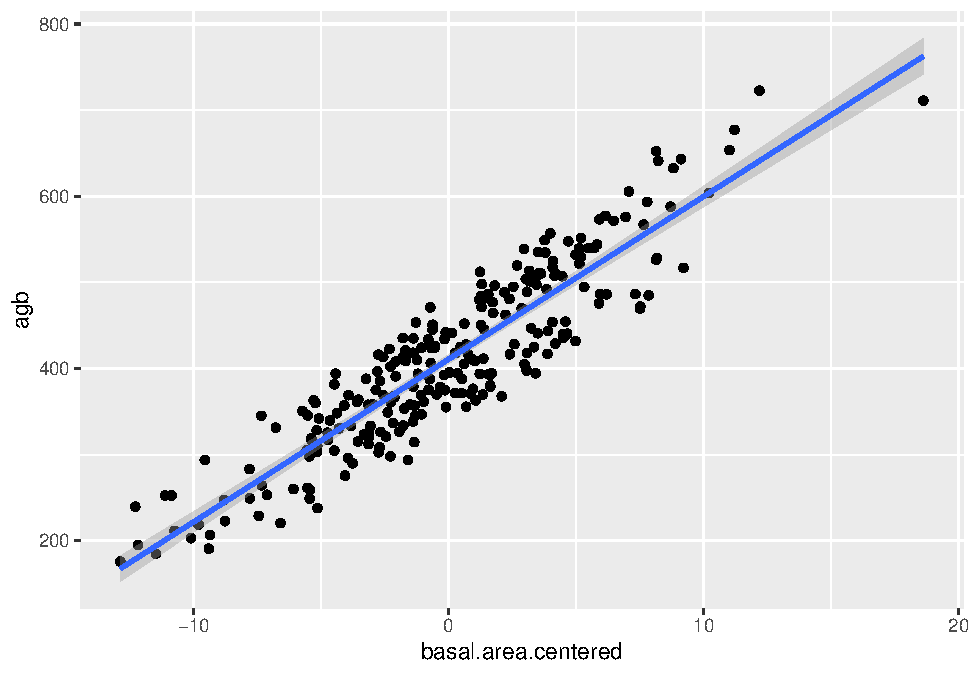
\includegraphics{Stats-Lab-7-FINAL_files/figure-latex/unnamed-chunk-8-1.pdf}

\hypertarget{question-4}{%
\subsection{Question 4}\label{question-4}}

Now suppose you wish to include both the difference between old-growth
forest and new-growth forest, as well as the effect of basal area on
AGB. y = beta0 + old.growthbeta1 + basal.area.centeredbeta2 + epsilon,
epsilon ∼ N (0, sigma2I). Call this model `fit\_4'.

\begin{Shaded}
\begin{Highlighting}[]
\NormalTok{fit\_4}\OtherTok{\textless{}{-}} \FunctionTok{lm}\NormalTok{(agb}\SpecialCharTok{\textasciitilde{}}\NormalTok{old.growth}\SpecialCharTok{+}\NormalTok{basal.area.centered, AGB.df)}
\FunctionTok{summary}\NormalTok{(fit\_4)}
\end{Highlighting}
\end{Shaded}

\begin{verbatim}
## 
## Call:
## lm(formula = agb ~ old.growth + basal.area.centered, data = AGB.df)
## 
## Residuals:
##     Min      1Q  Median      3Q     Max 
## -52.059 -15.138  -0.136  14.537  59.210 
## 
## Coefficients:
##                     Estimate Std. Error t value Pr(>|t|)    
## (Intercept)          374.399      2.017  185.60   <2e-16 ***
## old.growth            72.090      2.852   25.28   <2e-16 ***
## basal.area.centered   18.003      0.289   62.28   <2e-16 ***
## ---
## Signif. codes:  0 '***' 0.001 '**' 0.01 '*' 0.05 '.' 0.1 ' ' 1
## 
## Residual standard error: 22.38 on 247 degrees of freedom
## Multiple R-squared:  0.9527, Adjusted R-squared:  0.9523 
## F-statistic:  2488 on 2 and 247 DF,  p-value: < 2.2e-16
\end{verbatim}

\begin{enumerate}
\def\labelenumi{\alph{enumi}.}
\item
  What is the estimate of the intercept (beta0), and what does it
  represent in terms of AGB? \textgreater Answer: The estimate of beta0
  is 374.399. In terms of AGB, it represents the expected value of above
  ground biomass in new-growth forests with average basal area.
\item
  What is the estimate of beta1 and what does it represent in terms of
  AGB? \textgreater Answer: The estimate of beta1 is 72.090. In terms of
  AGB, it represents the expected difference in above ground biomass in
  new vs.~old growth forests with average basal area.
\item
  What is the estimate of beta2 and what does it represent in terms of
  AGB? \textgreater Answer: The estimate of beta2 18.003. In terms of
  AGB, it represents that for every 1 m\^{}2 increase in basal area,
  above ground biomass increases by 18.
\item
  Make a scatterplot of the data and add the regression lines. Follow
  the same color scheme used in question 2.
\end{enumerate}

\begin{Shaded}
\begin{Highlighting}[]
\FunctionTok{ggplot}\NormalTok{(AGB.df, }\FunctionTok{aes}\NormalTok{(}\AttributeTok{x=}\NormalTok{basal.area.centered, }\AttributeTok{y=}\NormalTok{agb, }\AttributeTok{color=}\NormalTok{old.growth))}\SpecialCharTok{+}\FunctionTok{geom\_point}\NormalTok{()}\SpecialCharTok{+}\FunctionTok{geom\_smooth}\NormalTok{(}\AttributeTok{method=}\NormalTok{lm, }\FunctionTok{aes}\NormalTok{(}\AttributeTok{group=}\NormalTok{old.growth, }\AttributeTok{color=}\NormalTok{old.growth))}
\end{Highlighting}
\end{Shaded}

\begin{verbatim}
## `geom_smooth()` using formula = 'y ~ x'
\end{verbatim}

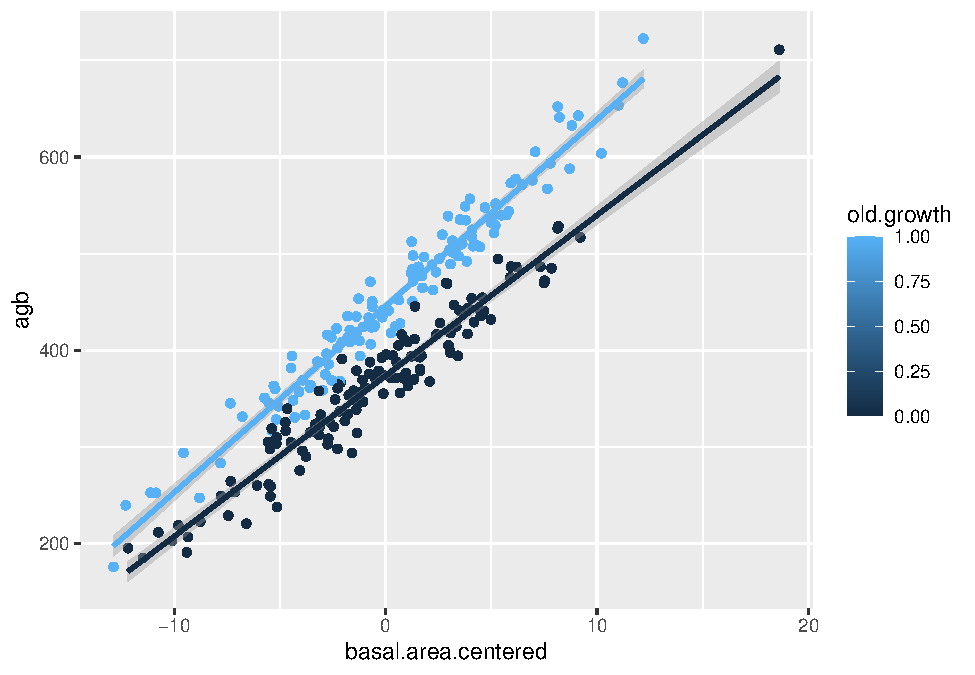
\includegraphics{Stats-Lab-7-FINAL_files/figure-latex/unnamed-chunk-10-1.pdf}

\begin{enumerate}
\def\labelenumi{\alph{enumi}.}
\setcounter{enumi}{4}
\tightlist
\item
  Comment on this plot? Do the results look reasonable? Does the slope
  of each regression line fit the data well? \textgreater Answer: On
  first glance, the results look reasonable. They show that old growth
  forests has higher AGB for a given basal area compared to new growth
  forests. The slope of each regression line fit the data well since
  R\^{}2 is very high, 0.9527. However, a few assumptions for regression
  may be slightly violated. The residuals vs fitted graph shows a slight
  banana shape so the assumption of linearity may be slightly violated.
  The points are fairly following the diagonal for the Q-Q residuals
  (only very slight deviations for values 182, 79 and 193) so no
  assumption is broken there. For the scale-location plot, it appears
  that the data points are well-distributed (with a slight bend upwards
  due to points 193 and 79) so the homoscedasticity assumption is met.
  In the residuals-leverage plot none of the values are beyond the
  dotted line representing Cook's distance, which suggests that while
  these values have a relatively strong influence, they are not
  outliers. When the shapiro.test for normalcy was run, the p-value is
  0.6063, which suggests that the assumption of normalcy is broken.
\end{enumerate}

\begin{Shaded}
\begin{Highlighting}[]
\FunctionTok{plot}\NormalTok{(fit\_4)}
\end{Highlighting}
\end{Shaded}

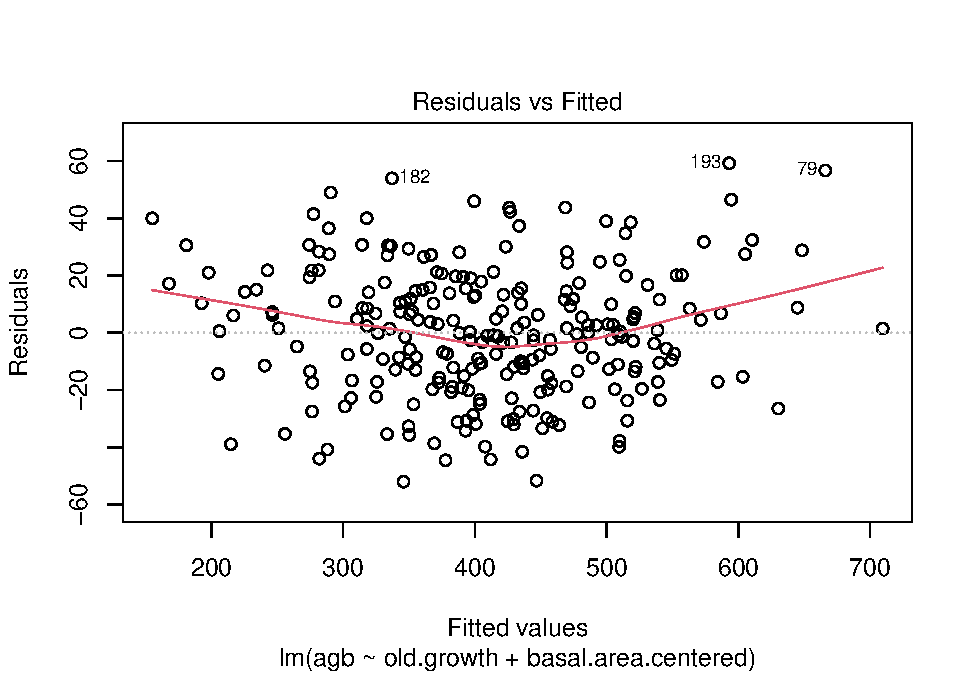
\includegraphics{Stats-Lab-7-FINAL_files/figure-latex/unnamed-chunk-11-1.pdf}
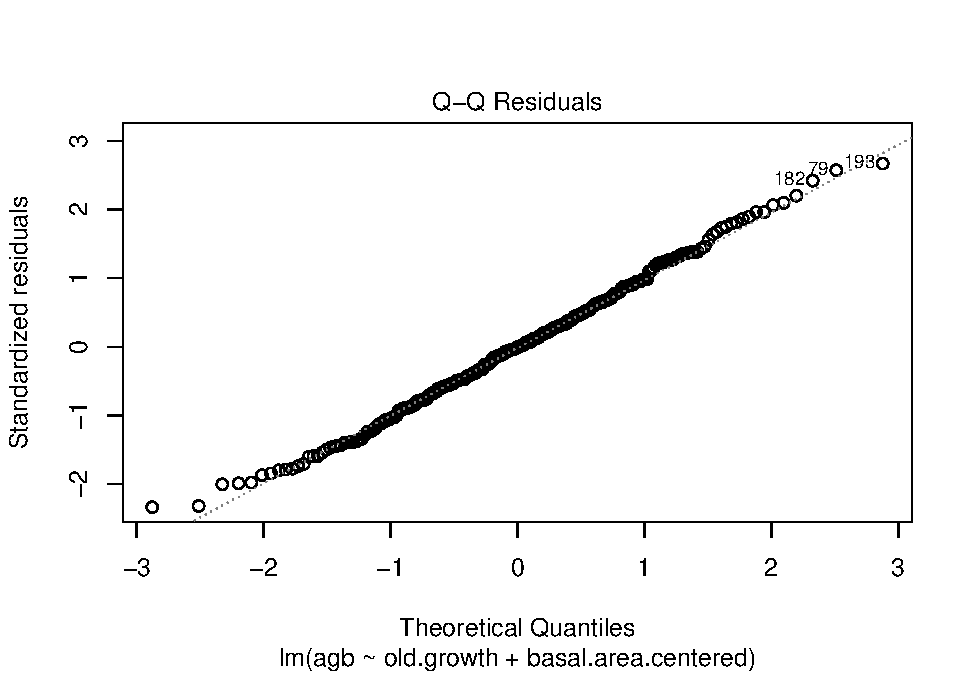
\includegraphics{Stats-Lab-7-FINAL_files/figure-latex/unnamed-chunk-11-2.pdf}
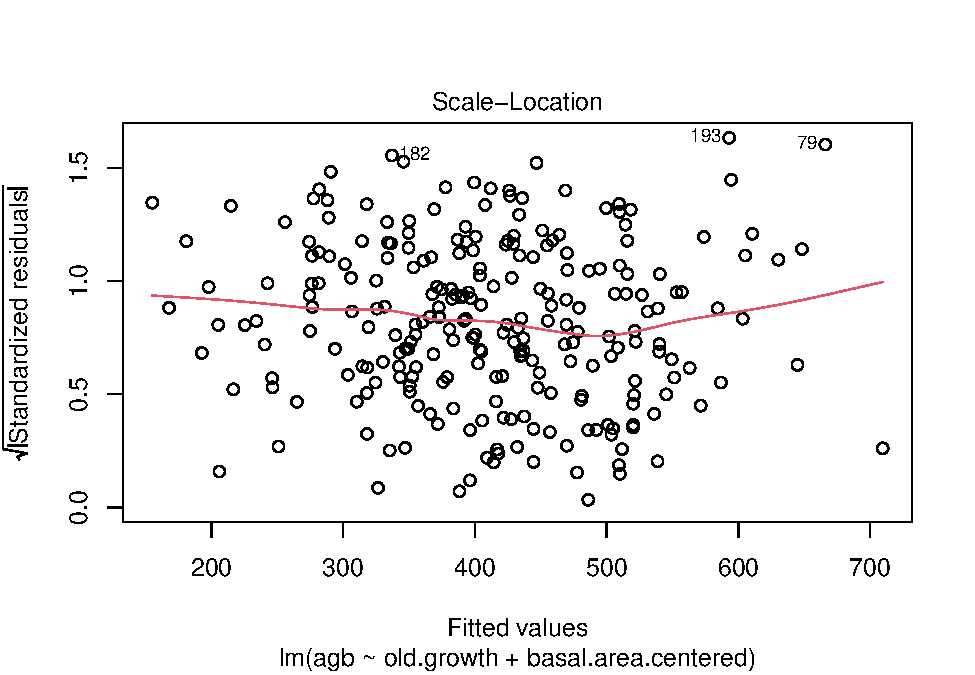
\includegraphics{Stats-Lab-7-FINAL_files/figure-latex/unnamed-chunk-11-3.pdf}
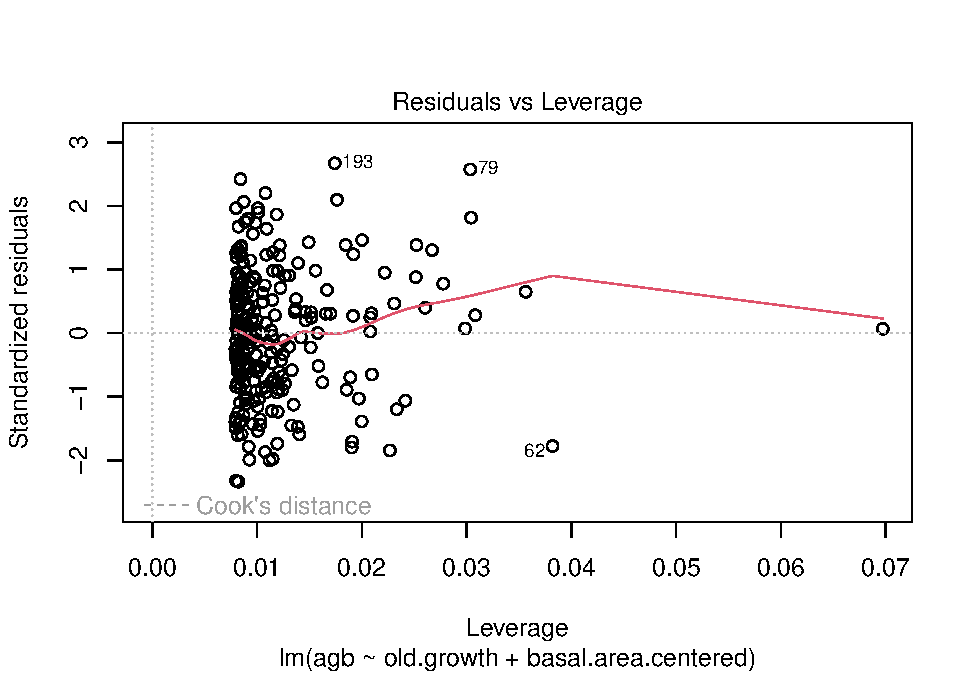
\includegraphics{Stats-Lab-7-FINAL_files/figure-latex/unnamed-chunk-11-4.pdf}

\begin{Shaded}
\begin{Highlighting}[]
\FunctionTok{shapiro.test}\NormalTok{(fit\_4}\SpecialCharTok{$}\NormalTok{residuals)}
\end{Highlighting}
\end{Shaded}

\begin{verbatim}
## 
##  Shapiro-Wilk normality test
## 
## data:  fit_4$residuals
## W = 0.99509, p-value = 0.6063
\end{verbatim}

\hypertarget{question-5}{%
\subsection{Question 5}\label{question-5}}

Now suppose you wish to test whether or not the effect of basal area
differs by old growth versus new growth. To do this, construct a new
covariate defined as `old.basal.area.centered' = `old.growth' ×
`basal.area.centered'. Now fit the following regression model: y = beta0
+ old.growthbeta1 + basal.area.centeredbeta2 +
old.basal.area.centeredbeta3 + epsilon, epsilon ∼ N (0, sigma2I). Call
this model `fit\_5'.

\begin{Shaded}
\begin{Highlighting}[]
\NormalTok{AGB.df}\OtherTok{\textless{}{-}}\NormalTok{AGB.df}\SpecialCharTok{\%\textgreater{}\%}
  \FunctionTok{mutate}\NormalTok{(}\AttributeTok{old.basal.area.centered =}\NormalTok{ old.growth}\SpecialCharTok{*}\NormalTok{basal.area.centered)}

\FunctionTok{colnames}\NormalTok{(AGB.df)}
\end{Highlighting}
\end{Shaded}

\begin{verbatim}
## [1] "growth"                  "state"                  
## [3] "basal_area"              "agb"                    
## [5] "old.growth"              "basal.area.centered"    
## [7] "old.basal.area.centered"
\end{verbatim}

\begin{Shaded}
\begin{Highlighting}[]
\NormalTok{fit\_5}\OtherTok{\textless{}{-}}\FunctionTok{lm}\NormalTok{(agb }\SpecialCharTok{\textasciitilde{}}\NormalTok{ old.growth }\SpecialCharTok{+}\NormalTok{ basal.area.centered }\SpecialCharTok{+}\NormalTok{ old.basal.area.centered, }\AttributeTok{data=}\NormalTok{ AGB.df)}

\FunctionTok{summary}\NormalTok{(fit\_5)}
\end{Highlighting}
\end{Shaded}

\begin{verbatim}
## 
## Call:
## lm(formula = agb ~ old.growth + basal.area.centered + old.basal.area.centered, 
##     data = AGB.df)
## 
## Residuals:
##     Min      1Q  Median      3Q     Max 
## -53.412 -14.763  -0.841  15.449  51.900 
## 
## Coefficients:
##                         Estimate Std. Error t value Pr(>|t|)    
## (Intercept)             373.5625     1.9398 192.578  < 2e-16 ***
## old.growth               72.1542     2.7316  26.415  < 2e-16 ***
## basal.area.centered      16.6245     0.3979  41.781  < 2e-16 ***
## old.basal.area.centered   2.6714     0.5540   4.822 2.49e-06 ***
## ---
## Signif. codes:  0 '***' 0.001 '**' 0.01 '*' 0.05 '.' 0.1 ' ' 1
## 
## Residual standard error: 21.43 on 246 degrees of freedom
## Multiple R-squared:  0.9568, Adjusted R-squared:  0.9563 
## F-statistic:  1816 on 3 and 246 DF,  p-value: < 2.2e-16
\end{verbatim}

\begin{enumerate}
\def\labelenumi{\alph{enumi}.}
\item
  What is the estimate of beta0 and what does it represent in terms of
  AGB? \textgreater Answer: The estimate of beta0 is 373.5625. This is
  the expected value of AGB in new-growth forests with average basal
  area.
\item
  What is the estimate of beta1 and what does it represent in terms of
  AGB? \textgreater Answer: The estimate of beta1 is 72.1542. This is
  the difference in expected value of AGB in new-growth forests
  vs.~old-growth forests with average basal area.
\item
  What is the estimate of beta2 and what does it represent in terms of
  AGB? \textgreater Answer: The estimate of beta2 is 16.6245. This is
  the expected change in AGB for each m\^{}2 increase in basal area
  among new-growth forests.
\item
  What is the estimate of beta3 and what does it represent in terms of
  AGB? \textgreater Answer: The estimate of beta3 is 2.6714. This is the
  adjustment to the slope for each m\^{}2 increase in basal area among
  old-growth forests.
\item
  Make a scatterplot of the data and add the regression lines. Follow
  the same color scheme used in questions 2 and 4.
\end{enumerate}

\begin{Shaded}
\begin{Highlighting}[]
\NormalTok{AGB.df}\OtherTok{\textless{}{-}}\NormalTok{AGB.df}\SpecialCharTok{\%\textgreater{}\%}
  \FunctionTok{mutate}\NormalTok{(}\AttributeTok{old.basal.area.centered =}\NormalTok{ old.growth}\SpecialCharTok{*}\NormalTok{basal.area.centered)}

\FunctionTok{colnames}\NormalTok{(AGB.df)}
\end{Highlighting}
\end{Shaded}

\begin{verbatim}
## [1] "growth"                  "state"                  
## [3] "basal_area"              "agb"                    
## [5] "old.growth"              "basal.area.centered"    
## [7] "old.basal.area.centered"
\end{verbatim}

\begin{Shaded}
\begin{Highlighting}[]
\NormalTok{fit\_5}\OtherTok{\textless{}{-}}\FunctionTok{lm}\NormalTok{(agb }\SpecialCharTok{\textasciitilde{}}\NormalTok{ old.growth }\SpecialCharTok{+}\NormalTok{ basal.area.centered }\SpecialCharTok{+}\NormalTok{ old.basal.area.centered, }\AttributeTok{data=}\NormalTok{ AGB.df)}

\FunctionTok{summary}\NormalTok{(fit\_5)}
\end{Highlighting}
\end{Shaded}

\begin{verbatim}
## 
## Call:
## lm(formula = agb ~ old.growth + basal.area.centered + old.basal.area.centered, 
##     data = AGB.df)
## 
## Residuals:
##     Min      1Q  Median      3Q     Max 
## -53.412 -14.763  -0.841  15.449  51.900 
## 
## Coefficients:
##                         Estimate Std. Error t value Pr(>|t|)    
## (Intercept)             373.5625     1.9398 192.578  < 2e-16 ***
## old.growth               72.1542     2.7316  26.415  < 2e-16 ***
## basal.area.centered      16.6245     0.3979  41.781  < 2e-16 ***
## old.basal.area.centered   2.6714     0.5540   4.822 2.49e-06 ***
## ---
## Signif. codes:  0 '***' 0.001 '**' 0.01 '*' 0.05 '.' 0.1 ' ' 1
## 
## Residual standard error: 21.43 on 246 degrees of freedom
## Multiple R-squared:  0.9568, Adjusted R-squared:  0.9563 
## F-statistic:  1816 on 3 and 246 DF,  p-value: < 2.2e-16
\end{verbatim}

\begin{Shaded}
\begin{Highlighting}[]
\FunctionTok{ggplot}\NormalTok{(AGB.df, }\FunctionTok{aes}\NormalTok{(}\AttributeTok{x=}\NormalTok{old.basal.area.centered, }\AttributeTok{y=}\NormalTok{agb))}\SpecialCharTok{+}\FunctionTok{geom\_point}\NormalTok{()}\SpecialCharTok{+}\FunctionTok{geom\_smooth}\NormalTok{(}\AttributeTok{method=}\NormalTok{lm)}
\end{Highlighting}
\end{Shaded}

\begin{verbatim}
## `geom_smooth()` using formula = 'y ~ x'
\end{verbatim}

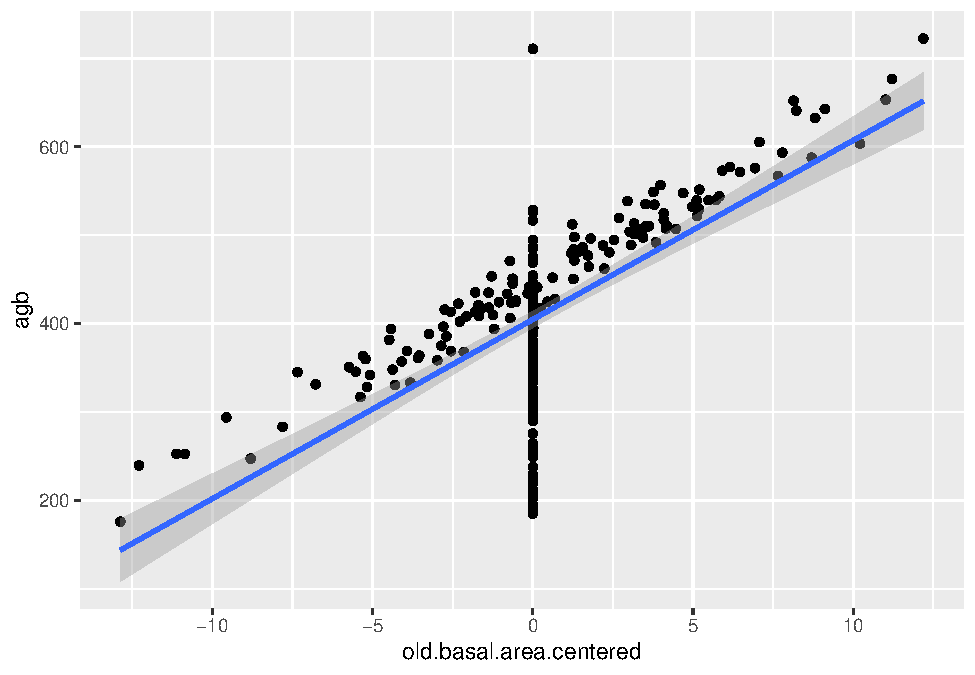
\includegraphics{Stats-Lab-7-FINAL_files/figure-latex/unnamed-chunk-13-1.pdf}

\begin{enumerate}
\def\labelenumi{\alph{enumi}.}
\setcounter{enumi}{5}
\tightlist
\item
  Comment on this plot. Do the results look reasonable? How does the
  plot compare to those from questions 3 and 4? \textgreater Answer: The
  results look reasonable as the regression assumptions have been met
  and this model seems to be good at explaining the variability of agb
  and old basal area centered (R-squared = 0.9568). The centerline in
  the residuals vs.~Fitted chart is fairly straight and in the middle so
  I think the linearity assumption is met. The Q-Q residuals line is
  fairly straight as well, with only a few data points at the tail end
  that deviate from the diagnoal line (values 182, 42 and 22). The
  scale-location graph shows that the plots are pretty well spread out
  so the homoscedasticity assumption is met. As for the residuals vs
  leverage graph, none of the data points are outside the dashed lines
  that represent Cook's distance so it is safe to assume that the data
  points, even point 233, is not influential enough to significantly
  shape the regression.
\end{enumerate}

\begin{Shaded}
\begin{Highlighting}[]
\FunctionTok{plot}\NormalTok{(fit\_5)}
\end{Highlighting}
\end{Shaded}

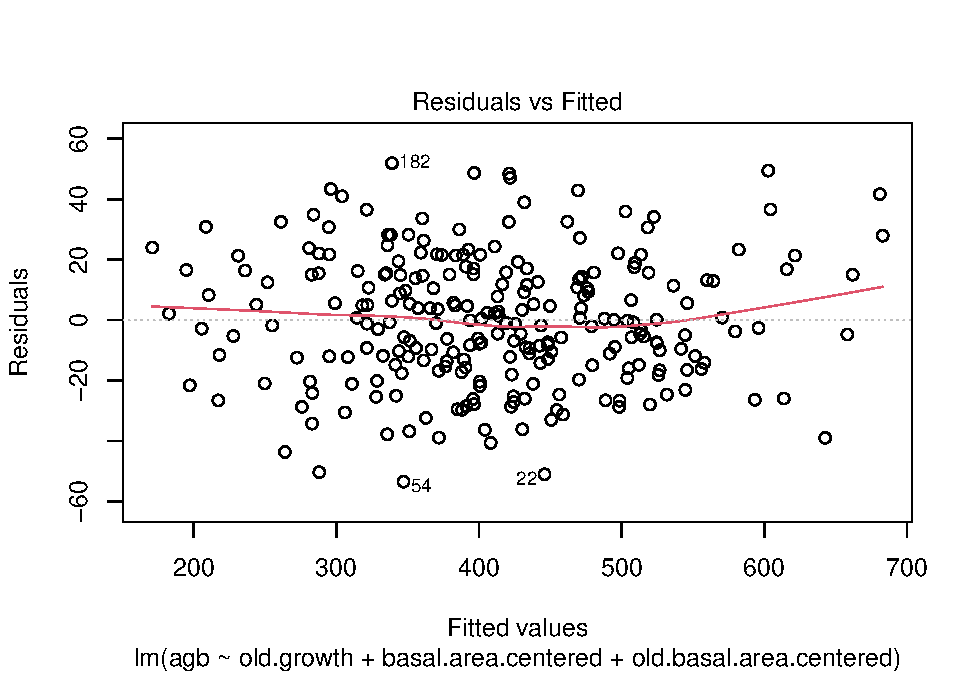
\includegraphics{Stats-Lab-7-FINAL_files/figure-latex/unnamed-chunk-14-1.pdf}
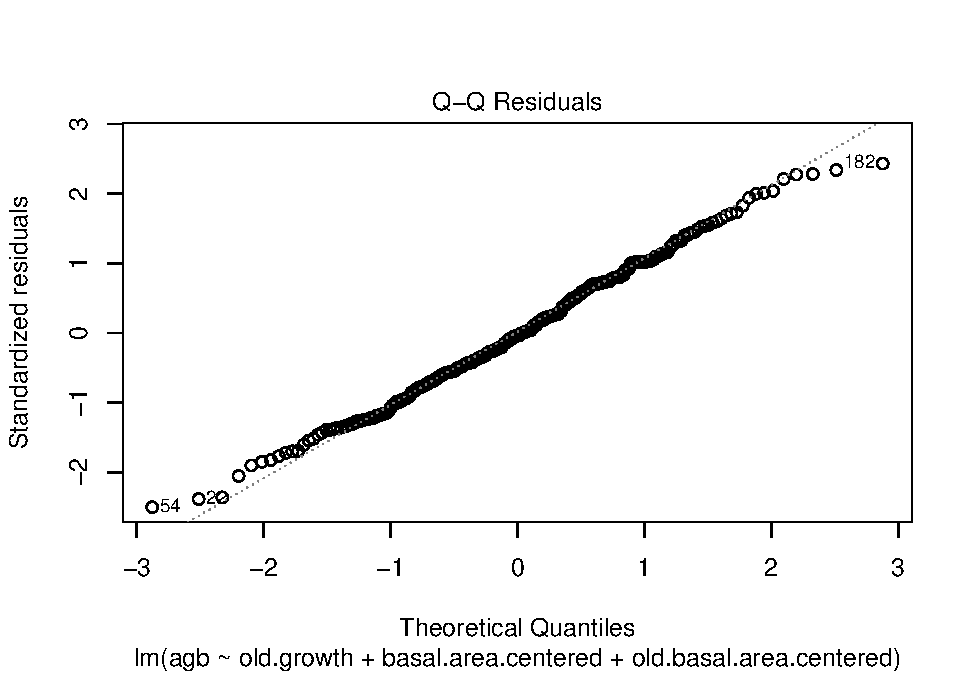
\includegraphics{Stats-Lab-7-FINAL_files/figure-latex/unnamed-chunk-14-2.pdf}
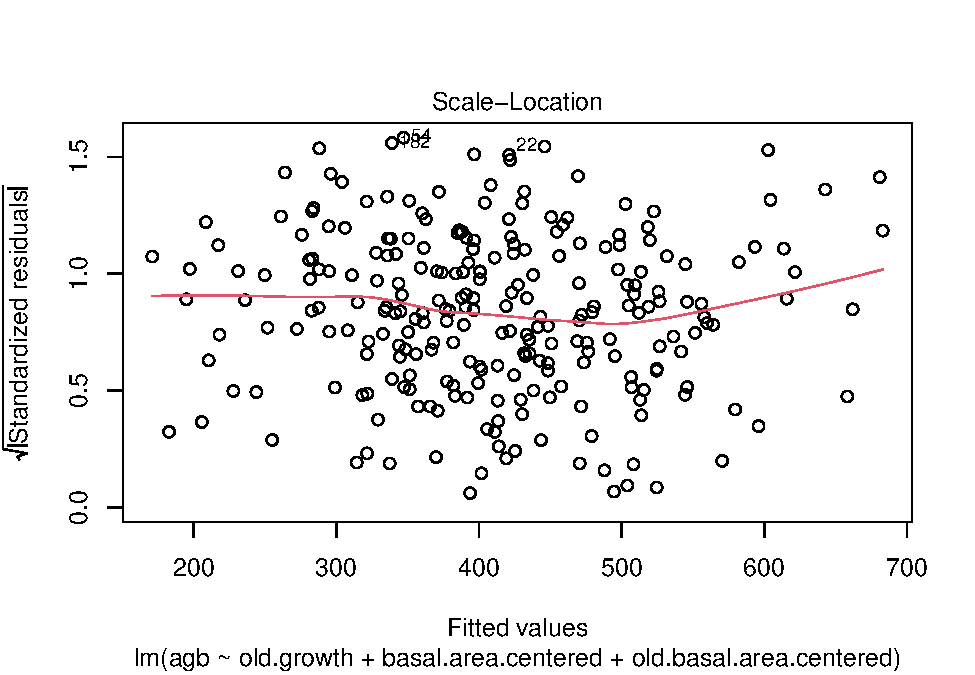
\includegraphics{Stats-Lab-7-FINAL_files/figure-latex/unnamed-chunk-14-3.pdf}
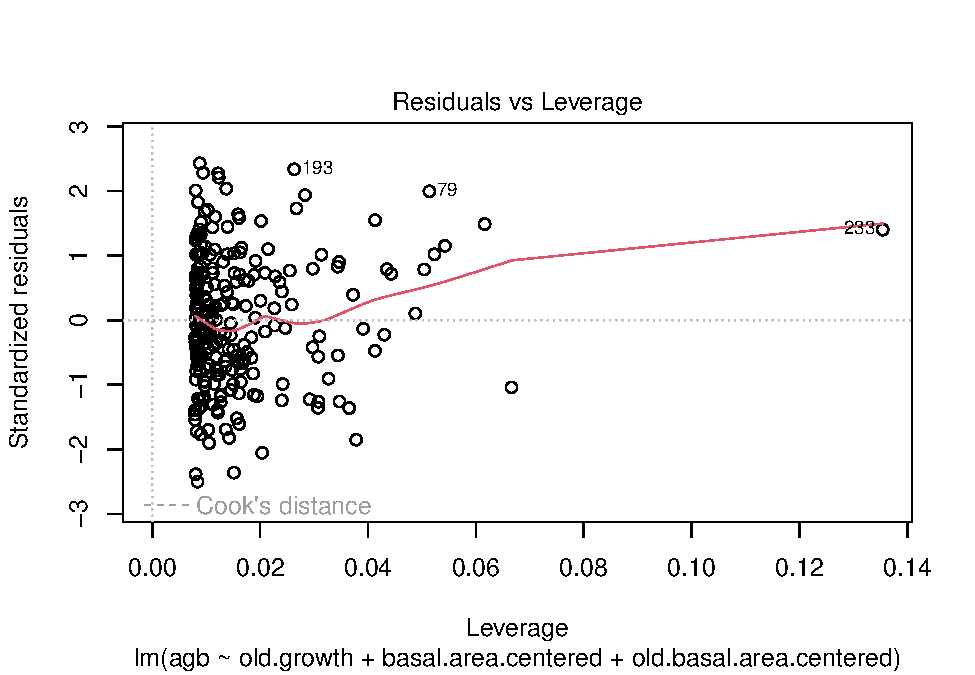
\includegraphics{Stats-Lab-7-FINAL_files/figure-latex/unnamed-chunk-14-4.pdf}

\begin{Shaded}
\begin{Highlighting}[]
\FunctionTok{shapiro.test}\NormalTok{(fit\_5}\SpecialCharTok{$}\NormalTok{residuals)}
\end{Highlighting}
\end{Shaded}

\begin{verbatim}
## 
##  Shapiro-Wilk normality test
## 
## data:  fit_5$residuals
## W = 0.99412, p-value = 0.4409
\end{verbatim}

\hypertarget{question-6}{%
\subsection{Question 6}\label{question-6}}

These data were collected from several different states
(CA,CO,ME,NC,WA). Suppose now you hypothesize that AGB varies by state.
To explore this, construct 4 binary indicator variables as follows:
`ca': code this variables as a 1 if the observation is from CA, and 0
otherwise `co': code this variables as a 1 if the observation is from
CO, and 0 otherwise `me': code this variables as a 1 if the observation
is from ME, and 0 otherwise `nc': code this variables as a 1 if the
observation is from NC, and 0 otherwise Now fit the following model: y =
beta0 + cabeta1 + cobeta2 + mebeta3 + ncbeta4 + epsilon, epsilon ∼ N (0,
sigma2I) Call this model `fit\_6'.

\begin{Shaded}
\begin{Highlighting}[]
\FunctionTok{colnames}\NormalTok{(AGB.df)}
\end{Highlighting}
\end{Shaded}

\begin{verbatim}
## [1] "growth"                  "state"                  
## [3] "basal_area"              "agb"                    
## [5] "old.growth"              "basal.area.centered"    
## [7] "old.basal.area.centered"
\end{verbatim}

\begin{Shaded}
\begin{Highlighting}[]
\FunctionTok{head}\NormalTok{(AGB.df}\SpecialCharTok{$}\NormalTok{state)}
\end{Highlighting}
\end{Shaded}

\begin{verbatim}
## [1] "CA" "WA" "ME" "NC" "CA" "CA"
\end{verbatim}

\begin{Shaded}
\begin{Highlighting}[]
\NormalTok{AGB.df}\OtherTok{\textless{}{-}}\NormalTok{ AGB.df}\SpecialCharTok{\%\textgreater{}\%}
  \FunctionTok{mutate}\NormalTok{(}\AttributeTok{ca =} \FunctionTok{ifelse}\NormalTok{(state }\SpecialCharTok{==}\StringTok{"CA"}\NormalTok{,}\DecValTok{1}\NormalTok{,}\DecValTok{0}\NormalTok{))}\SpecialCharTok{\%\textgreater{}\%}
  \FunctionTok{mutate}\NormalTok{(}\AttributeTok{co =} \FunctionTok{ifelse}\NormalTok{(state }\SpecialCharTok{==}\StringTok{"CO"}\NormalTok{,}\DecValTok{1}\NormalTok{,}\DecValTok{0}\NormalTok{))}\SpecialCharTok{\%\textgreater{}\%}
  \FunctionTok{mutate}\NormalTok{(}\AttributeTok{me =} \FunctionTok{ifelse}\NormalTok{(state }\SpecialCharTok{==}\StringTok{"ME"}\NormalTok{,}\DecValTok{1}\NormalTok{,}\DecValTok{0}\NormalTok{))}\SpecialCharTok{\%\textgreater{}\%}
  \FunctionTok{mutate}\NormalTok{(}\AttributeTok{nc =} \FunctionTok{ifelse}\NormalTok{(state }\SpecialCharTok{==}\StringTok{"NC"}\NormalTok{,}\DecValTok{1}\NormalTok{,}\DecValTok{0}\NormalTok{))}

\NormalTok{fit\_6}\OtherTok{\textless{}{-}} \FunctionTok{lm}\NormalTok{(agb}\SpecialCharTok{\textasciitilde{}}\NormalTok{ca}\SpecialCharTok{+}\NormalTok{co}\SpecialCharTok{+}\NormalTok{me}\SpecialCharTok{+}\NormalTok{nc, }\AttributeTok{data=}\NormalTok{AGB.df) }
\FunctionTok{summary}\NormalTok{(fit\_6)}
\end{Highlighting}
\end{Shaded}

\begin{verbatim}
## 
## Call:
## lm(formula = agb ~ ca + co + me + nc, data = AGB.df)
## 
## Residuals:
##      Min       1Q   Median       3Q      Max 
## -237.293  -69.268   -7.507   71.261  286.304 
## 
## Coefficients:
##             Estimate Std. Error t value Pr(>|t|)    
## (Intercept)   411.75      15.06  27.346   <2e-16 ***
## ca             16.34      20.14   0.811    0.418    
## co            -32.11      20.39  -1.575    0.117    
## me             24.54      20.47   1.199    0.232    
## nc            -18.35      21.81  -0.842    0.401    
## ---
## Signif. codes:  0 '***' 0.001 '**' 0.01 '*' 0.05 '.' 0.1 ' ' 1
## 
## Residual standard error: 101 on 245 degrees of freedom
## Multiple R-squared:  0.04448,    Adjusted R-squared:  0.02888 
## F-statistic: 2.851 on 4 and 245 DF,  p-value: 0.02447
\end{verbatim}

\begin{enumerate}
\def\labelenumi{\alph{enumi}.}
\item
  What is the estimate of the beta0 and what does it represent in terms
  of AGB? \textgreater Answer: The estimate of beta0 is 411.75 and this
  is the expected AGB in WA.
\item
  What is the estimate of beta1 and what does it represent in terms of
  AGB? \textgreater Answer: The estimate of beta1 is 16.34 and this is
  the difference in expected AGB between WA and CA, holding all else
  constant.
\item
  What is the estimate of beta2 and what does it represent in terms of
  AGB? \textgreater Answer: The estimate of beta2 is -32.11 and this is
  the difference in expected AGB between WA and CO, holding all else
  constant.
\item
  What is the estimate of beta3 and what does it represent in terms of
  AGB? \textgreater Answer: The estimate of beta3 is 24.54 and this is
  the difference in expected AGB between WA and ME, holding all else
  constant.
\item
  What is the estimate of beta4 and what does it represent in terms of
  AGB? \textgreater Answer: The estimate of beta4 is -18.35 and this is
  the difference in expected AGB between WA and NC, holding all else
  constant.
\item
  Make a scatterplot of the data (with states on the x-axis and AGB on
  the y-axis) and plot the regression lines. As before, color the data
  points and regression lines by state.
\end{enumerate}

\begin{Shaded}
\begin{Highlighting}[]
\FunctionTok{ggplot}\NormalTok{(}\AttributeTok{data=}\NormalTok{ AGB.df, }\FunctionTok{aes}\NormalTok{(}\AttributeTok{x=}\NormalTok{state, }\AttributeTok{y=}\NormalTok{agb, }\AttributeTok{color=}\NormalTok{state))}\SpecialCharTok{+}\FunctionTok{geom\_point}\NormalTok{()}
\end{Highlighting}
\end{Shaded}

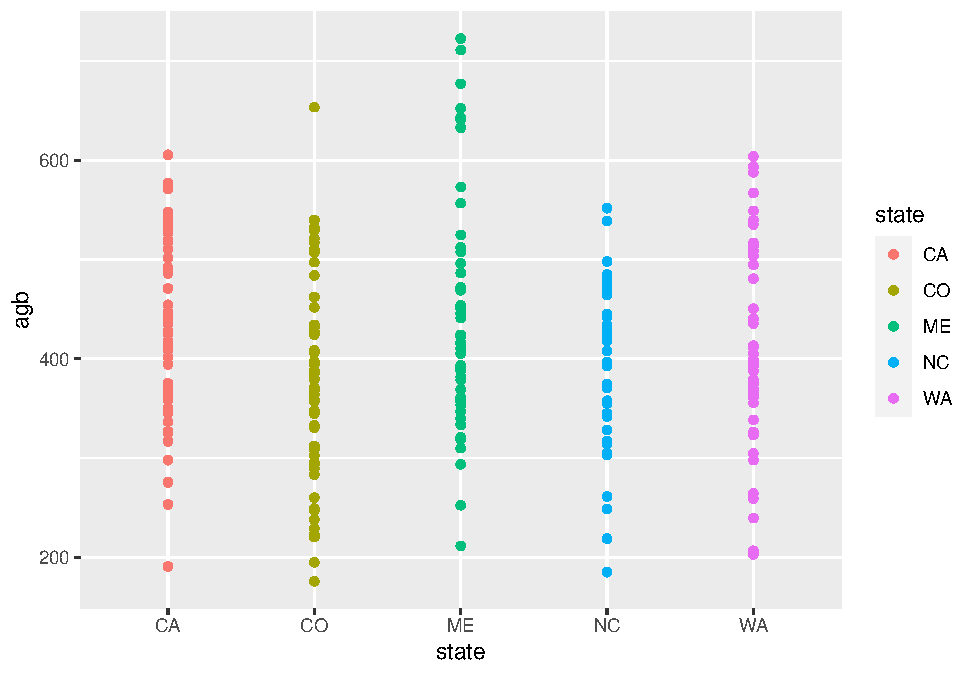
\includegraphics{Stats-Lab-7-FINAL_files/figure-latex/unnamed-chunk-15-1.pdf}

\begin{Shaded}
\begin{Highlighting}[]
\CommentTok{\#Need to add regression lines}
\end{Highlighting}
\end{Shaded}

\begin{enumerate}
\def\labelenumi{\alph{enumi}.}
\setcounter{enumi}{6}
\tightlist
\item
  Comment on this plot? Based on the plot and the results from the
  model, does there appear to be variability in AGB by state?
  \textgreater Answer: With p-value of 0.02888, there seems to be
  statistically significant variability in AGB by state. Based on the
  R-squared value, 4.448\% of the variation can be explained by this
  model, which suggests that other variables need to be taken into
  account. When testing for the regression assumptions, it appears that
  the assumption of normalcy in distribution of residuals is violated
  because the p-value is quite high (0.444). However, looking at the
  residuals vs leverage graph, it appears that none of the data points
  can be considered outliers since all are within Cook's distance. The
  data points on the Q-Q residuals plot are fairly straight, and so are
  the center lines for the Residuals vs.~Fitted and Scale location
  graphs.
\end{enumerate}

\begin{Shaded}
\begin{Highlighting}[]
\FunctionTok{plot}\NormalTok{(fit\_6)}
\end{Highlighting}
\end{Shaded}

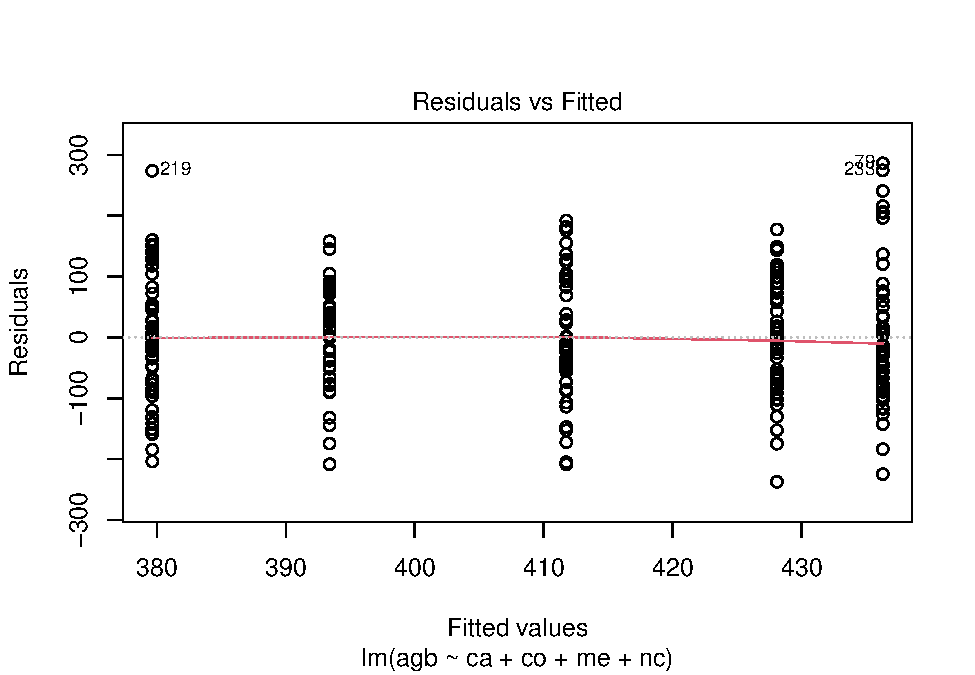
\includegraphics{Stats-Lab-7-FINAL_files/figure-latex/unnamed-chunk-16-1.pdf}
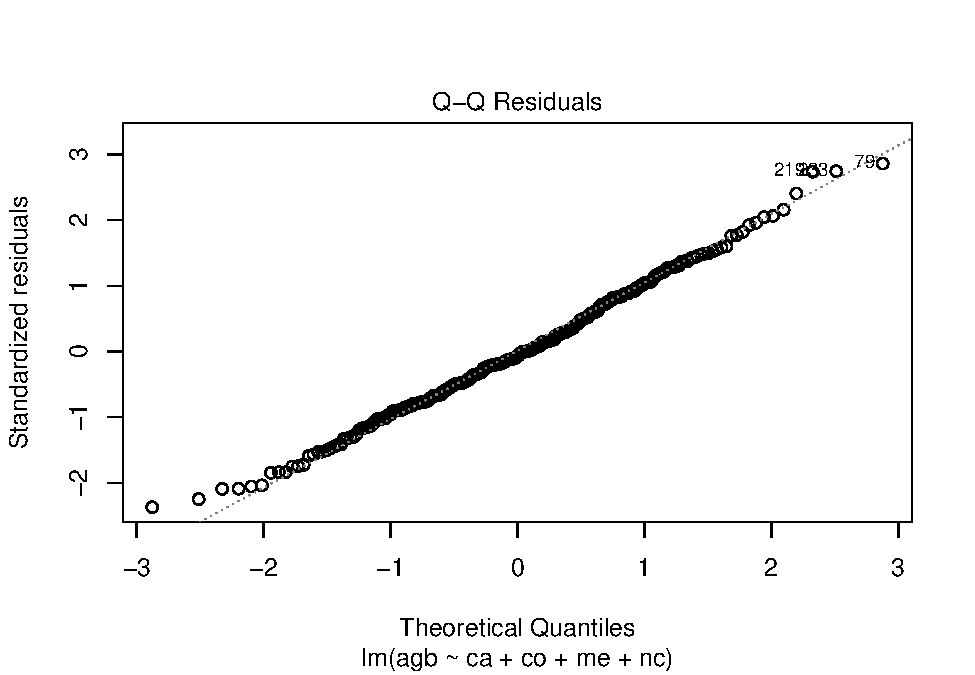
\includegraphics{Stats-Lab-7-FINAL_files/figure-latex/unnamed-chunk-16-2.pdf}
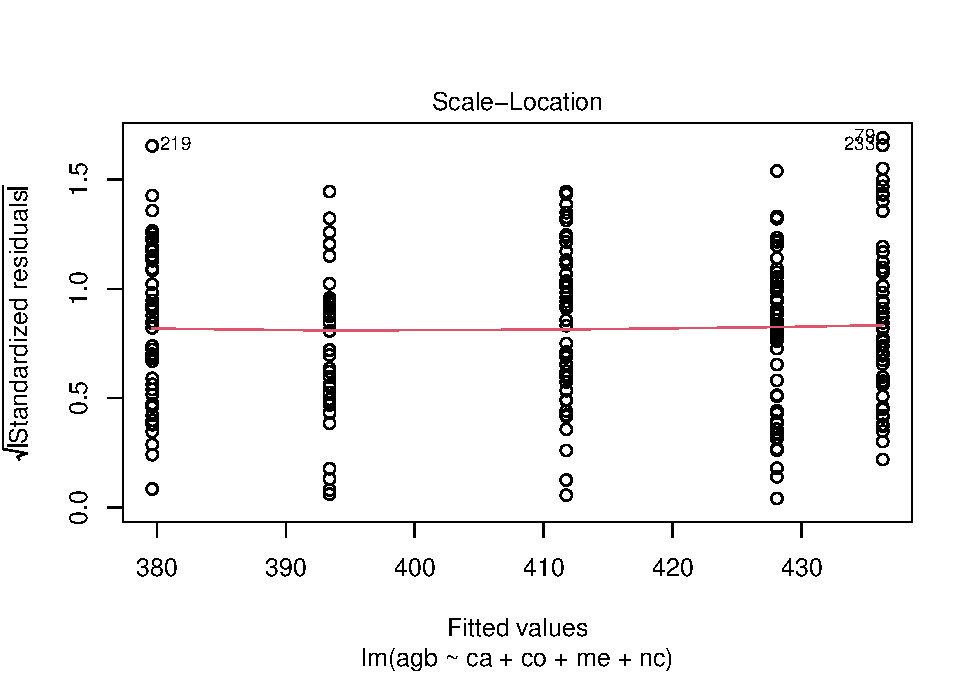
\includegraphics{Stats-Lab-7-FINAL_files/figure-latex/unnamed-chunk-16-3.pdf}
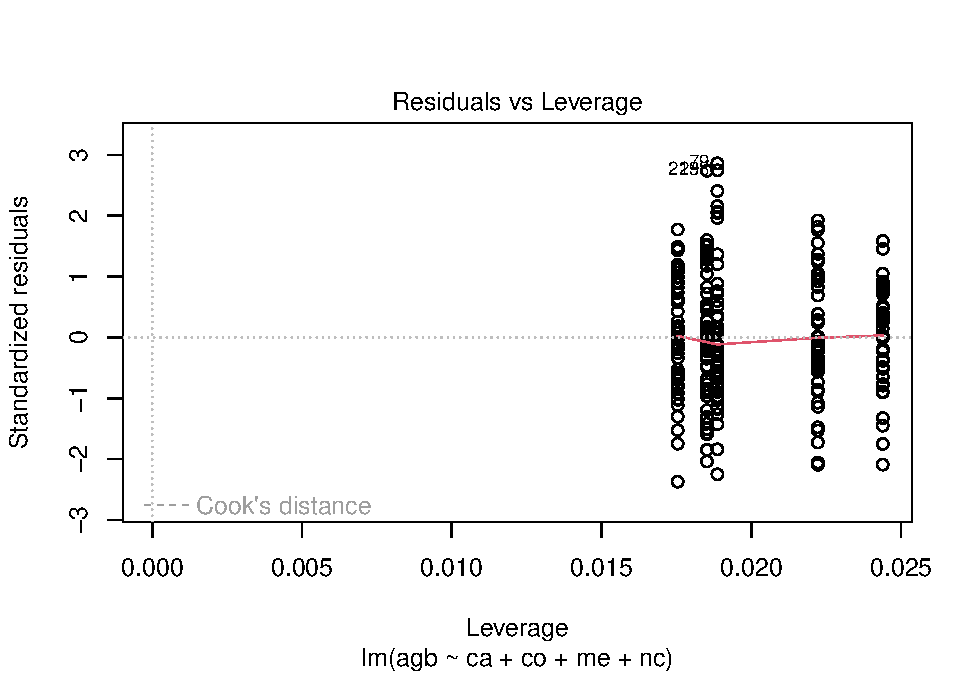
\includegraphics{Stats-Lab-7-FINAL_files/figure-latex/unnamed-chunk-16-4.pdf}

\begin{Shaded}
\begin{Highlighting}[]
\FunctionTok{shapiro.test}\NormalTok{(fit\_6}\SpecialCharTok{$}\NormalTok{residuals)}
\end{Highlighting}
\end{Shaded}

\begin{verbatim}
## 
##  Shapiro-Wilk normality test
## 
## data:  fit_6$residuals
## W = 0.99414, p-value = 0.444
\end{verbatim}

\end{document}
